\documentclass{article}
\usepackage[utf8]{inputenc}
\usepackage{amsmath,amsthm,amssymb}
\usepackage{graphicx}
\usepackage{parskip}

\newcommand{\code}[1]{\texttt{#1}}

\begin{document}

\title{%
	CTA200 Assignment 2 \\[0.3cm]
	\large Winter 2020}
\author{Jeff Shen}
\date{\today}

\maketitle

\section*{Question 1}

\begin{figure}[!htbp]
	\centering
	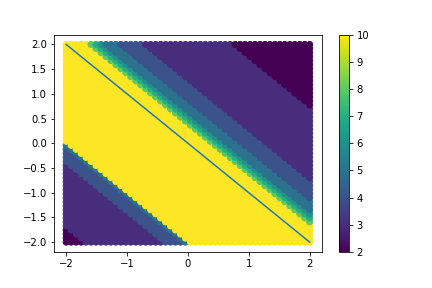
\includegraphics[width=0.8\linewidth]{q1.png}
\end{figure}

\subsection*{Methods}

Basic numerical packages were imported in Python, which were used for this and the next question. Two 1D arrays, each sampling 50 points from -2 to 2, were created. One was multiplied by \code{1j} in order to make it an array of complex values. Using these two arrays, \code{np.meshgrid} was used to create a grid of (50, 50) points in the appropriate range. The array was flattened into a (50x50, 1) shape, which then served as \code{c} from the question. 10 iterations was the maximum number that does not cause an overflow, and so that is the number that was selected. Each new column was created with the equation $z_{i+1} = z_i^2 + c$ according to the instructions, where each $z$ and each $c$ is a column of 50x50 values. The iteration number at which a given point diverged was calculated by setting a divergence threshold of where the 2D \code{z} array was greater than 10. This didn't seem to differ much with a threshold of 1000. These numbers seem reasonable since they are greater than $|z|^2$ would be for convergent values. Then, a mask was created with \code{np.where}, which indicated the iteration number for when some row (representing a single $c$ value) crossed the threshold. The original (50, 50) grid was then plotted using matplotlib, with the iteration number set as the colour. 

\subsection*{Analysis}

asdf

\newpage 

\section*{Question 2}

\begin{figure}[!htbp]
	\centering
	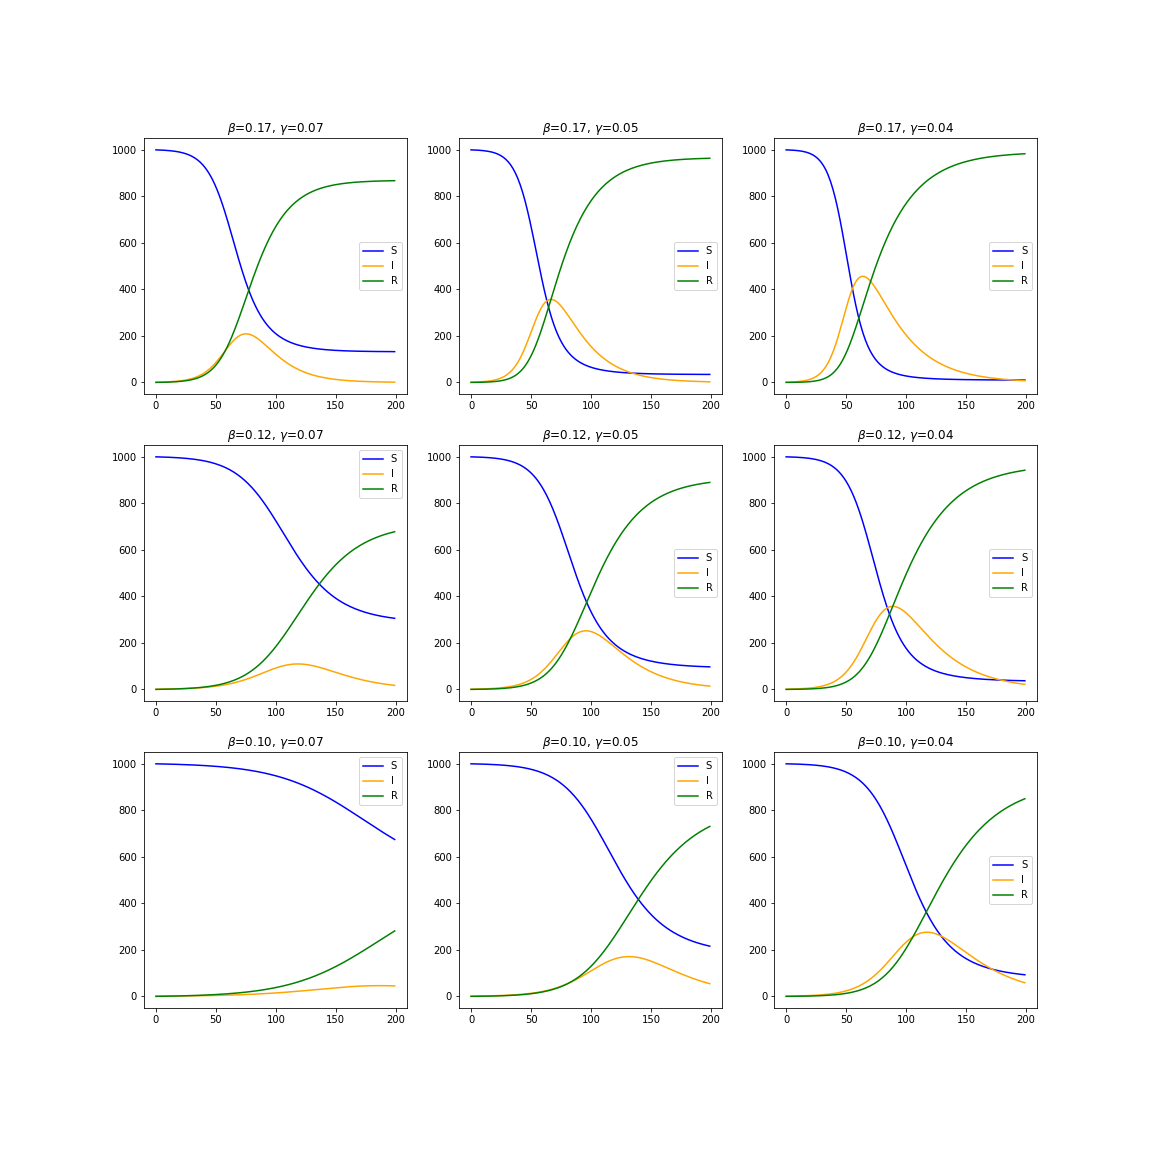
\includegraphics[width=1.2\linewidth]{q2.png}
\end{figure}

\subsection*{Methods}

\code{odeint} was imported from \code{scipy}. A derivatives function was created: it takes parameters y (a tuple of S, I, and R), t (array for integration time), $\beta$, $\gamma$, and N, and returns the derivatives $dS/dt$, $dI/dt$, and $dR/dt$ according to the appropriate ODEs. The initial conditions were set according to the instructions. $1/\beta$ is the expected number of days it takes for an infected person to infect one other person, and the values $1/6$, $1/8$, and $1/10$ were selected for $\beta$ (ie. 6 days to infect someone else, etc.). $1/\gamma$ is the number of days it takes for an infected person to recover, and the values of $1/14$, $1/21$, and $1/28$ were selected for $\gamma$ (ie. it takes 2 weeks to recover, etc.). I'm not an epidemiologist and have no experience with disease modelling, but these numbers don't seem wildly unreasonable. For each combination of parameters, the ODE integrator integrated all the way to $t=200$, and the S, I, and R lines were plotted. In the resulting 3x3 grid of plots, each row has the same $\beta$ value, and each column has the same $\gamma$ value. 

\subsection*{Analysis}

asdf

\end{document}
